\section{问题一模型的建立与求解}
\subsection{数据预处理}

附件 1 的数据以 10 min 为间隔，故将一天划分为 144 个调度时段，每段长度 \(\Delta t=\frac{1}{6}\ \mathrm{h}\)；
原始时间标签表示该时段的开始时刻，例如“00:10”对应 \([00:10,00:20)\)。

附件 1 的电价具有明显的日内波动：全天共出现 137 个不同价格，最低 \(0.3713\) 元/kWh（05:30—05:40），
最高 \(1.3952\) 元/kWh（20:30—20:40），峰谷价差 \(1.0239\) 元/kWh。因此不宜以全天购电量最小为目标，
而应以全天购电费用最低为目标。光伏出力集中在白天，约 04:30 后开始上升、19:20 左右降至零，
全天最大预测功率 \(7612.32\ \mathrm{kW}\)（12:00—12:10）；144 个时段中有 30 个时段光伏功率高于同期负载，
这部分富余电能需由储能消纳。储能最大容量 12000 kWh，实际运行储电量保持在 \(1200\sim10800\ \mathrm{kWh}\)，
最大充放电功率 5000 kW。结合电价峰谷差，储能在吸收白天富余光伏之外，还可在低价时段购电充电、
高价时段放电，从而降低全天购电费用。

综上，问题一的实质是在负荷需求、储能容量与充放电功率约束下，对外网购电、光伏利用与储能充放电
进行合理分配，实现全天购电费用最小。

\subsection{构建混合整数线性规划模型}

设 \(t=1,2,\ldots,144\) 为时段编号，\(L_t\)、\(PV_t\)、\(\pi_t\) 分别为该时段的小区负载功率、
光伏预测功率与外网电价。光伏优先供给负载，据此先构造三个不需要优化的辅助量：
光伏直供负载功率 \(PV_t^{L}=\min(PV_t,L_t)\)、光伏供电后的负荷缺口
\(\overline L_t=\max(L_t-PV_t,0)\)、满足负载后的富余光伏 \(\overline{PV}_t=\max(PV_t-L_t,0)\)。

决策变量为：外网直接供负载功率 \(G_t^L\)、外网用于储能充电的功率 \(G_t^{ch}\)、
光伏用于储能充电的功率 \(PV_t^{ch}\)、储能充放电功率 \(C_t,D_t\)、时段末储电量 \(E_t\)、
弃光功率 \(V_t\) 以及充放电状态二元变量 \(u_t\)。外网总购电功率由
\(G_t=G_t^L+G_t^{ch}\) 派生，以便直接追踪每一单位外网电的去向。

\subsubsection{目标函数}

全天购电费用为各时段购电费用之和，目标函数为

\begin{equation}
\min Z=
\sum_{t=1}^{144}
\pi_t
\left(G_t^L+G_t^{ch}\right)\Delta t.
\end{equation}

其中 \(Z\) 表示全天总购电费用。

\subsubsection{约束条件}

\textbf{1、负荷供电约束}

微网提供的电能不得低于小区负载，光伏供电后的剩余负荷由外网与储能共同承担：

\begin{equation}
G_t^L+D_t=\overline L_t.
\end{equation}

\textbf{2、储能充电来源约束}

储能设备的充电功率可以由富余光伏和外部电网共同提供，因此有 \(PV_t^{ch}+G_t^{ch}=C_t\)。 且满足 \(0\leq PV_t^{ch}\leq\overline{PV}_t,, G_t^{ch}\geq0\)。 \textbf{3、光伏剩余功率约束}

剩余光伏优先用于储能充电，受容量与功率限制无法消纳的部分记为弃光：

\begin{equation}
PV_t^{ch}+V_t=\overline{PV}_t,
\end{equation}

其中 \(V_t\geq0\)。 \textbf{4、储能电量变化约束}

题目给出充放电效率为 90\%，本文取 \(\eta_c=\eta_d=0.90\)，相邻时段储电量满足

\begin{equation}
E_t
=
E_{t-1}
+\eta_cC_t\Delta t
-\frac{D_t\Delta t}{\eta_d}.
\end{equation}

\textbf{5、储能容量约束}

储电量运行区间为 1200～10800 kWh：

\begin{equation}
1200\leq E_t\leq10800.
\end{equation}

题目要求 0:00 与 24:00 储电量相同，取 \(E_0=6000\ \mathrm{kWh}\)，故有 \(E_{144}=E_0=6000\)。 \textbf{6、储能充放电功率约束}

充放电功率不超过 5000 kW：

\[
0\leq C_t\leq5000,
\]

\begin{equation}
0\leq D_t\leq5000.
\end{equation}

\textbf{7、储能充放电互斥约束}

同一时段储能不能同时充电和放电，故引入二元变量 \(u_t\)（\(u_t=1\) 允许充电，\(u_t=0\) 允许放电）：

\[
C_t\leq5000u_t,
\]

\[
D_t\leq5000(1-u_t),
\]

\begin{equation}
u_t\in\{0,1\}.
\end{equation}

综合上述条件，问题一的优化模型如下：

\begin{equation}
\boxed{
\begin{aligned}
\min\quad
&Z=\sum_{t=1}^{144}
\pi_t(G_t^L+G_t^{ch})\Delta t \\[1mm]
{\rm s.t.}\quad
&G_t^L+D_t=\overline L_t,\\
&PV_t^{ch}+G_t^{ch}=C_t,\\
&PV_t^{ch}+V_t=\overline{PV}_t,\\
&E_t=E_{t-1}
+\eta_cC_t\Delta t
-\frac{D_t\Delta t}{\eta_d},\\
&1200\leq E_t\leq10800,\\
&E_0=E_{144}=6000,\\
&0\leq C_t\leq5000,\\
&0\leq D_t\leq5000,\\
&C_t\leq5000u_t,\\
&D_t\leq5000(1-u_t),\\
&u_t\in\{0,1\}.
\end{aligned}}
\end{equation}

至此，问题一被转化为一个含有连续变量和二进制变量的混合整数线性规划问题。

\subsection{模型求解}

由前面我们建立的模型可以得到，外网直接供负载功率 \(G_t^L\)、外网充电功率 \(G_t^{ch}\)、光伏充电功率 \(PV_t^{ch}\)、储能充电功率 \(C_t\)、储能放电功率 \(D_t\)、储电量 \(E_t\) 和弃光功率 \(V_t\) 均为连续变量，而用于刻画储能充放电状态的 \(u_t\) 为 0-1 变量。因此，该模型属于混合整数线性规划模型。

由于一天被划分为 144 个 10 min 调度时段，每个时段包含 7 个连续变量和 1 个二元变量，因此模型共有 \(144\times 8=1152\) 个决策变量，其中连续变量 1008 个，0-1 整数变量 144 个。

针对该类含有离散决策变量的线性优化问题，我们采用分支定界法进行求解。其基本思想是：首先暂时放松整数约束，将二元变量 \(u_t\in\{0,1\}\) 放宽为 \(0\leq u_t\leq1\)， 求解得到原混合整数规划问题的线性规划松弛解；若所得 \(u_t\) 均满足整数条件，则该解即为当前节点的整数可行解。若存在部分 \(u_t\) 取非整数值，则选取相应变量进行分支，将原问题划分为若干规模更小的子问题，并分别计算各子问题的目标函数下界。在不断进行“分支—求界—剪枝”的过程中，逐步缩小整数最优解可能存在的搜索区域，直至得到全局最优解。

具体求解过程如下。

\subsubsection{分支定界法的实现}

问题一模型含 1152 个决策变量（1008 个连续变量与 144 个 0-1 变量），采用分支定界法求解。
基本思想是先把 0-1 变量松弛为连续变量求 LP 松弛解：若松弛解中所有 \(u_t\) 均取 0 或 1，
它同时满足整数约束，即为原问题最优解；否则选取取分数值的 \(u_k\) 分支，把问题划分为
\(u_k=0\) 与 \(u_k=1\) 两个子问题，分别求其 LP 松弛值作为该节点的下界，再用
不可行剪枝（子问题无可行解）与界剪枝（节点下界已不低于当前最好整数解）删除不可能
产生更优解的节点，同时用切平面收紧可行域。当搜索中取得满足整数约束的可行解时更新上界，
上下界逐步逼近，直至收敛。

对最小化问题，全程满足

\[
LB\leq Z^*\leq UB,
\]

其中 \(LB\) 为剩余节点的最小下界，\(UB\) 为当前最好整数解的目标值，\(Z^*\) 为原问题真实最优值。
定义绝对最优间隙

\[
Gap=UB-LB,
\]

当不存在尚未处理且可能产生更优解的节点，或间隙满足收敛条件时，即认为当前整数可行解达到全局最优。

\subsubsection{程序实现}

本文利用 MATLAB 建立混合整数线性规划模型并调用 \texttt{intlinprog} 求解：先读入 144 个时段的
电价、负荷与光伏数据，按式（3）计算光伏直供功率、剩余负荷与富余光伏；随后写入目标函数系数、
三类能量流向平衡约束、储能状态递推、储电量上下限、充放功率限制与充放电互斥条件，
并将 \(u_t\) 指定为整数变量。求解器采用 LP 松弛热启动，再对非整数变量分支，
通过节点下界、整数上界与切平面逐步缩小搜索空间。

\subsubsection{求解结果}

根据分支定界法所得最优结果，全天计划购电量为 \(\boxed{59482.70\ \mathrm{kWh}}\)， 全天最小购电费用为 \(\boxed{35126.95\ \mathrm{元}}\)。 全天储能累计充电量为 \(20740.67\ \mathrm{kWh}\)， 累计放电量为 \(16799.94\ \mathrm{kWh}\)。 储能设备在 0:00 时的电量为 \(6000\ \mathrm{kWh}\)， 在全天调度结束后的 24:00 储电量仍为 \(6000\ \mathrm{kWh}\)， 满足题目要求的首末储电量相同条件。

同时，全天弃光量为 \(0.00\ \mathrm{kWh}\)， 说明优化策略能够将当天产生的富余光伏全部通过负荷直接消纳或储能充电的方式加以利用。

在数值检验中，模型三类流量平衡约束的最大残差不超过 \(4.5\times10^{-13}\)，储能状态转移约束的最大残差约为 \(1.48\times10^{-12}\)， 均接近计算机浮点计算精度范围。由此说明求得的最优解在数值上严格满足负荷平衡、光伏分配以及储能状态转移等约束条件，所得计划购电策略具有较好的可靠性。

%FIG:BEGIN q1-day
典型日的分时电价与逐 10 min 计划购电量对照见图~\ref{fig:q1-day}。

\begin{figure}[htbp]
\centering
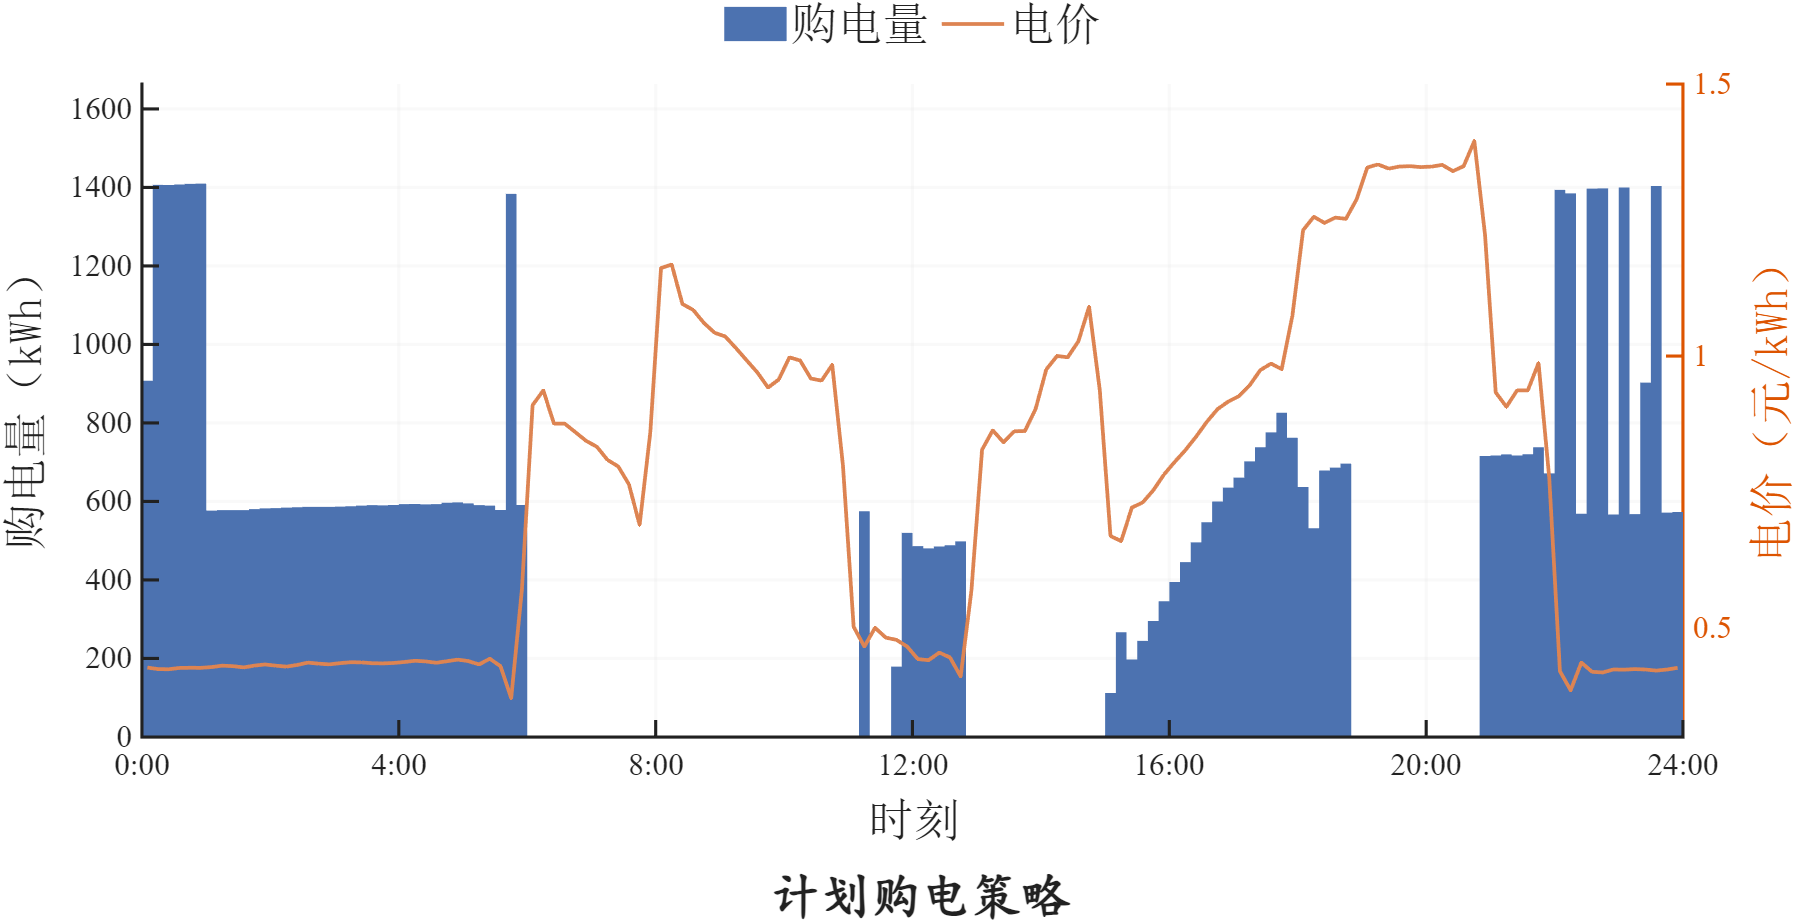
\includegraphics[width=0.78\textwidth,height=0.26\textheight,keepaspectratio]{figures/q1_day_plan.png}
\caption{典型日的分时电价与逐 10 min 计划购电量（电价单位：元/kWh，购电量单位：kWh）}
\label{fig:q1-day}
\end{figure}

计划购电量与电价呈反向分布，全天 144 个时段中有 58 个时段购电量为零，二者相关系数为 $-0.555$。若按 00:00—01:00 与 22:00—24:00 计谷段（占时长 12.5\%），该段承担了 33.7\% 的购电量，而 18:00—21:00 晚峰仅占 6.6\%，可见储能把购电从高价时段搬到了低价时段。
%FIG:END q1-day

%FIG:BEGIN q1-soc
储能设备的充放电量与储电量变化见图~\ref{fig:q1-soc}。

\begin{figure}[htbp]
\centering

\includegraphics[width=0.78\textwidth,height=0.26\textheight,keepaspectratio]{figures/q1_soc.png}
\caption{典型日储能充放电量与储电量（电量单位：kWh）}
\label{fig:q1-soc}
\end{figure}

全天充电量 20\,740.67 kWh、放电量 16\,799.94 kWh，储电量始终落在 $[1200,\ 10800]$ kWh 的运行区间内。充电量大于放电量是充放电效率均为 0.90 的正常结果，并非计算误差。
%FIG:END q1-soc
%MANDATED:BEGIN
按题目表 1 与表 2 要求的格式，将上述结果整理见下页横版表。

\begin{landscape}
\vspace*{-1.4\baselineskip}
\begin{center}{\heiti\zihao{4}问题一：指定时间段购电量与储能充放电量（题目表 1、表 2 格式）}\end{center}
\vspace{0.1\baselineskip}
{\zihao{6}
\noindent
\begin{minipage}[t]{0.485\linewidth}
\begin{tabular}{|c|r|c|r|c|r|}
\hline
时间段 & 购电量/kWh & 时间段 & 购电量/kWh & 时间段 & 购电量/kWh \\
\hline
10:00-10:10 & \textbf{0.00} & 12:00-12:10 & \textbf{520.12} & 14:00-14:10 & \textbf{0.00} \\
\hline
16:00-16:10 & \textbf{345.78} & 18:00-18:10 & \textbf{762.42} & 20:00-20:10 & \textbf{0.00} \\
\hline
全天购电量 & \textbf{59482.70} & & & 全天购电费 & \textbf{35126.95} \\
\hline
\end{tabular}
\par\vspace{2pt}{\zihao{6}（a）微网在指定时间段的购电量及全天的购电量和购电费}

\end{minipage}\hfill
\begin{minipage}[t]{0.485\linewidth}
\begin{tabular}{|c|r|r|c|r|r|}
\hline
时间段 & 充电量/kWh & 放电量/kWh & 时间段 & 充电量/kWh & 放电量/kWh \\
\hline
0:00-4:00 & \textbf{4500.00} & \textbf{0.00} & 4:00-8:00 & \textbf{833.33} & \textbf{5947.42} \\
\hline
8:00-12:00 & \textbf{3954.63} & \textbf{2121.42} & 12:00-16:00 & \textbf{6119.37} & \textbf{91.10} \\
\hline
16:00-20:00 & \textbf{0.00} & \textbf{5068.69} & 20:00-24:00 & \textbf{5333.33} & \textbf{3571.31} \\
\hline
0:00 储电量 & \textbf{6000.00} & & 24:00 储电量 & \textbf{6000.00} & \\
\hline
\end{tabular}
\par\vspace{2pt}{\zihao{6}（b）储能设备在指定时间段的充放电量及 0:00 和 24:00 的储电量}

\end{minipage}
}
\end{landscape}


%MANDATED:END

\subsection{结论分析}

综合以上分析，可以得到如下结论：在满足小区负载、储能运行区间、最大充放电功率以及首末储电量一致等约束条件下，模型能够合理协调光伏发电、外网购电和储能设备之间的电能分配。

首先，购电量与外网电价总体呈现明显的反向变化关系，其相关系数为 \(-0.555\)。 其中，00:00—01:00 和 22:00—24:00 两个低价时段合计仅占全天时间的 \(12.5\%\)，但购电量约占全天总购电量的 \(31.8\%\)；而 18:00—21:00 的高电价时段购电量仅占全天的 \(6.8\%\)。说明优化模型主动将部分购电行为从高价时段转移到了低价时段。

其次，储能设备具有明显的“谷充峰放”特征。00:00—01:00 时段累计充电约 4166.67 kWh；在早间电价较高的 06:00—08:00 时段累计放电约 7201 kWh；19:00—20:00 晚高峰时段累计放电约 7120 kWh。整个调度过程中储电量能够达到 10800 kWh 的上限和 1200 kWh 的下限，说明储能设备的可利用容量得到了充分发挥。

最后，为分析储能装置对购电成本的影响，令储能设备不进行任何充放电，即 \(C_t=D_t=0\)， 得到无储能情况下的基准结果。此时全天购电量为 \(61789.94\ \mathrm{kWh}\)， 全天购电费用为 \(48052.05\ \mathrm{元}\)。 采用本文最优调度策略后，全天购电量降低至 59482.70 kWh，仅减少约 \(3.73\%\)， 但购电费用降低至 35126.95 元，节约 \(12925.10\ \mathrm{元}\)， 降幅达到 \(\boxed{26.90\%}\)。 因此可以看出，储能设备带来的经济效益并不主要来源于减少总购电量，而主要来自低电价时段购电、高电价时段放电所形成的峰谷电价套利。同时，模型实现全天零弃光，使光伏发电得到了充分利用。
